%!TEX program = lualatex
\documentclass[11pt,class=beamer]{standalone}
\usepackage{etoolbox}
\usepackage{ifxetex}
\usepackage{ifluatex}
\usepackage[T1]{fontenc}
\ifboolexpr{bool{xetex} or bool{luatex}}{%
	\usepackage{fontspec}
}{%
	\usepackage[utf8]{inputenc}
}
\usepackage{xcolor}

\usepackage{amsmath}
\usepackage{amssymb}
\usepackage{mathrsfs}
\usepackage{braket}

\usepackage{pgf}
\usepackage{tikz}
\usepackage{tikzpeople}

\usepackage{array}
\usepackage{tabularx}
\usepackage{multirow}

\usetikzlibrary{shapes}
\usetikzlibrary{arrows.meta}
\usetikzlibrary{calc}
\usetikzlibrary{positioning}
\usetikzlibrary{angles}
\usetikzlibrary{quotes}
\usetikzlibrary{decorations}

\definecolor{bg_color}{RGB}{250,250,229}
\definecolor{Cblue}{RGB}{38,75,150}
\definecolor{Cgreen}{RGB}{39,179,118}
\definecolor{Cdarkgreen}{RGB}{0,111,60}
\definecolor{Corange}{RGB}{249,167,62}
\definecolor{Cred}{RGB}{191,33,47}

\colorlet{good}{green!90!black}
\colorlet{average}{Corange}
\colorlet{bad}{Cred}


\beamertemplatenavigationsymbolsempty{}

\begin{document}
	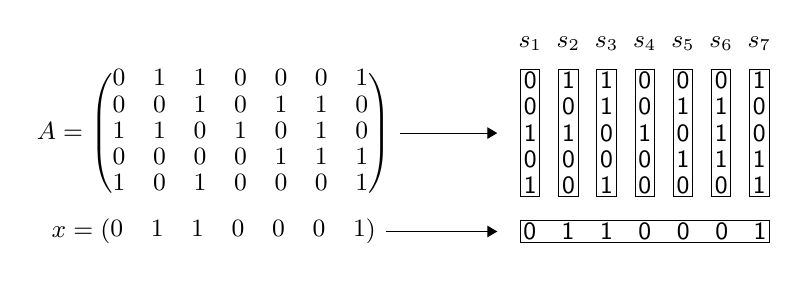
\begin{tikzpicture}[
		x=1pt,
		y=1pt,
		/utils/exec={\sffamily},
		font=\fontsize{9pt}{9.5pt}\selectfont,
		>=Triangle,
		decoration={snake,segment length=5,amplitude=0.7},
	]
		\tikzset{bitset/.style={
			draw,
			rectangle,
			inner sep=1,
			outer sep=3.4,
			text width=5,
			text centered,
		}}
		\tikzset{bitseth/.style={
			draw,
			rectangle,
			inner sep=1,
			outer sep=3.4,
		}}

		\node (A) at (0,0) {\(A = \begin{pmatrix}
			0 & 1 & 1 & 0 & 0 & 0 & 1 \\
			0 & 0 & 1 & 0 & 1 & 1 & 0 \\
			1 & 1 & 0 & 1 & 0 & 1 & 0 \\
			0 & 0 & 0 & 0 & 1 & 1 & 1 \\
			1 & 0 & 1 & 0 & 0 & 0 & 1 \\
		\end{pmatrix}\)};

		\node[anchor=north] (x) at (A.south) {\(x = \begin{pmatrix}
			0 & 1 & 1 & 0 & 0 & 0 & 1
		\end{pmatrix}\)};


		\node[
			bitset,
			anchor=west,
			xshift=40,
		] (bitset1) at (A.east) {0\\0\\1\\0\\1};
		\node[
			bitset,
			anchor=west,
		] (bitset2) at (bitset1.east) {1\\0\\1\\0\\0};
		\node[
			bitset,
			anchor=west,
		] (bitset3) at (bitset2.east) {1\\1\\0\\0\\1};
		\node[
			bitset,
			anchor=west,
		] (bitset4) at (bitset3.east) {0\\0\\1\\0\\0};
		\node[
			bitset,
			anchor=west,
		] (bitset5) at (bitset4.east) {0\\1\\0\\1\\0};
		\node[
			bitset,
			anchor=west,
		] (bitset6) at (bitset5.east) {0\\1\\1\\1\\0};
		\node[
			bitset,
			anchor=west,
		] (bitset7) at (bitset6.east) {1\\0\\0\\1\\1};

		\node[anchor=south] at (bitset1.north) {\(s_1\)};
		\node[anchor=south] at (bitset2.north) {\(s_2\)};
		\node[anchor=south] at (bitset3.north) {\(s_3\)};
		\node[anchor=south] at (bitset4.north) {\(s_4\)};
		\node[anchor=south] at (bitset5.north) {\(s_5\)};
		\node[anchor=south] at (bitset6.north) {\(s_6\)};
		\node[anchor=south] at (bitset7.north) {\(s_7\)};

		\draw[->] (A) -- ($(bitset1.west)-(5,0)$);

		\node[
			bitseth,
			anchor=west,
		] (bitsetx) at (x.west -| bitset1.south west) {0\ \ \ 1\ \ \ 1\ \ \ 0\ \ \ 0\ \ \ 0\ \ \ 1};

		\draw[->] (x) -- ($(bitsetx.west)-(5,0)$);
	\end{tikzpicture}%
\end{document}%